\documentclass{beamer}

\usepackage[utf8]{inputenc}
\usepackage[T2A]{fontenc}
\usepackage[english,russian]{babel}
\usepackage[normalem]{ulem}


\usepackage{tikz}
\usetikzlibrary{arrows,decorations.pathmorphing,backgrounds,fit,positioning,shapes,shapes.symbols,chains}

\usetheme{Frankfurt}

% Переведем заголовки блоков на русский
\uselanguage{russian}
\languagepath{russian}
\deftranslation[to=russian]{Theorem}{Теорема}
\deftranslation[to=russian]{Example}{Пример}


% \usefonttheme{professionalfonts}
\usefonttheme{serif}
% \usefonttheme{structureitalicserif}


\DeclareMathOperator*{\minn}{min}
\DeclareMathOperator*{\argmin}{argmin}

\begin{document}

\title{Оптимизация транспортного потока при заданных пунктах отправления и назначения всех участников движения}
\author{Пехтерев С.И. 610 группа\\Научный руководитель: д.ф.-м.н. Васенин В.А.}
\institute[]{}
\date[16.05.2022]{16 мая 2022}

% Создание заглавной страницы
% \frame{\titlepage}
\maketitle


% % Автоматическая генерация содержания
% \frame{
%   \frametitle{План}
%   \tableofcontents
% }

\section{Задача кооперативной оптимизации транспортного потока}

\begin{frame}\frametitle{Основные определения}
  \begin{itemize}
	\item   \emph{Дорожной сетью} назовем тройку $G = (V, E, l)$, где $(V, E)$ --- ориентированный граф с длинами ребер $l: E \rightarrow \mathbb{R}_{>0} $.
	
	\item Предположим, что имеется $n$ участников с заданными точками отправления $A_i \in V$ и прибытия $B_i \in V$. Пусть множество $P_i$ есть множество всех простых путей из $A_i$ в $B_i$. Элемент декартового произведения ${P = \prod \limits_{i = 1} ^ n P_i}$ назовем \emph{комбинацией путей}.
	
	\item Пусть известно, что при комбинации путей участников $\textbf{p} = \left(p_1, \ldots, p_n\right)\in P$ $i$-ый участник затрачивает $T_i(\textbf{p}) \in \mathbb{R}_{\ge 0}$ времени на свой путь.  Функции $T_i$ назовем \textit{функциями временных затрат} участника $i$.
\end{itemize}
\end{frame}

\begin{frame}\frametitle{Некооперативное прокладывание пути}
  
  \textit{Некооперативным прокладыванием пути} в дорожной сети $G$ назовем пятерку $F = (n, G, \{A_i\}_{i = 1}^{n}, \{B_i\}_{i = 1}^{n}, \{T_i\}_{i = 1}^{n})$. Некооперативное прокладывание пути предполагает, что каждый участник стремится сократить собственные временные затраты выбором пути $p_i$, несмотря на временные затраты других участников.

\bigskip
Равновесие Нэша: ни одному из участников невыгодно изменение его маршрута.
  
\end{frame}

\begin{frame}\frametitle{Парадокс Браеса}
	Равновесие Нэша может не соответствовать оптимальному решению. Пусть из A в B отправляется $4\,000$ участников, а время проезда по ребру зависит от числа участников (метка на ребре).
	
	\begin{figure}[H]
		\begin{center}
			\begin{minipage}[h]{0.45\linewidth}
				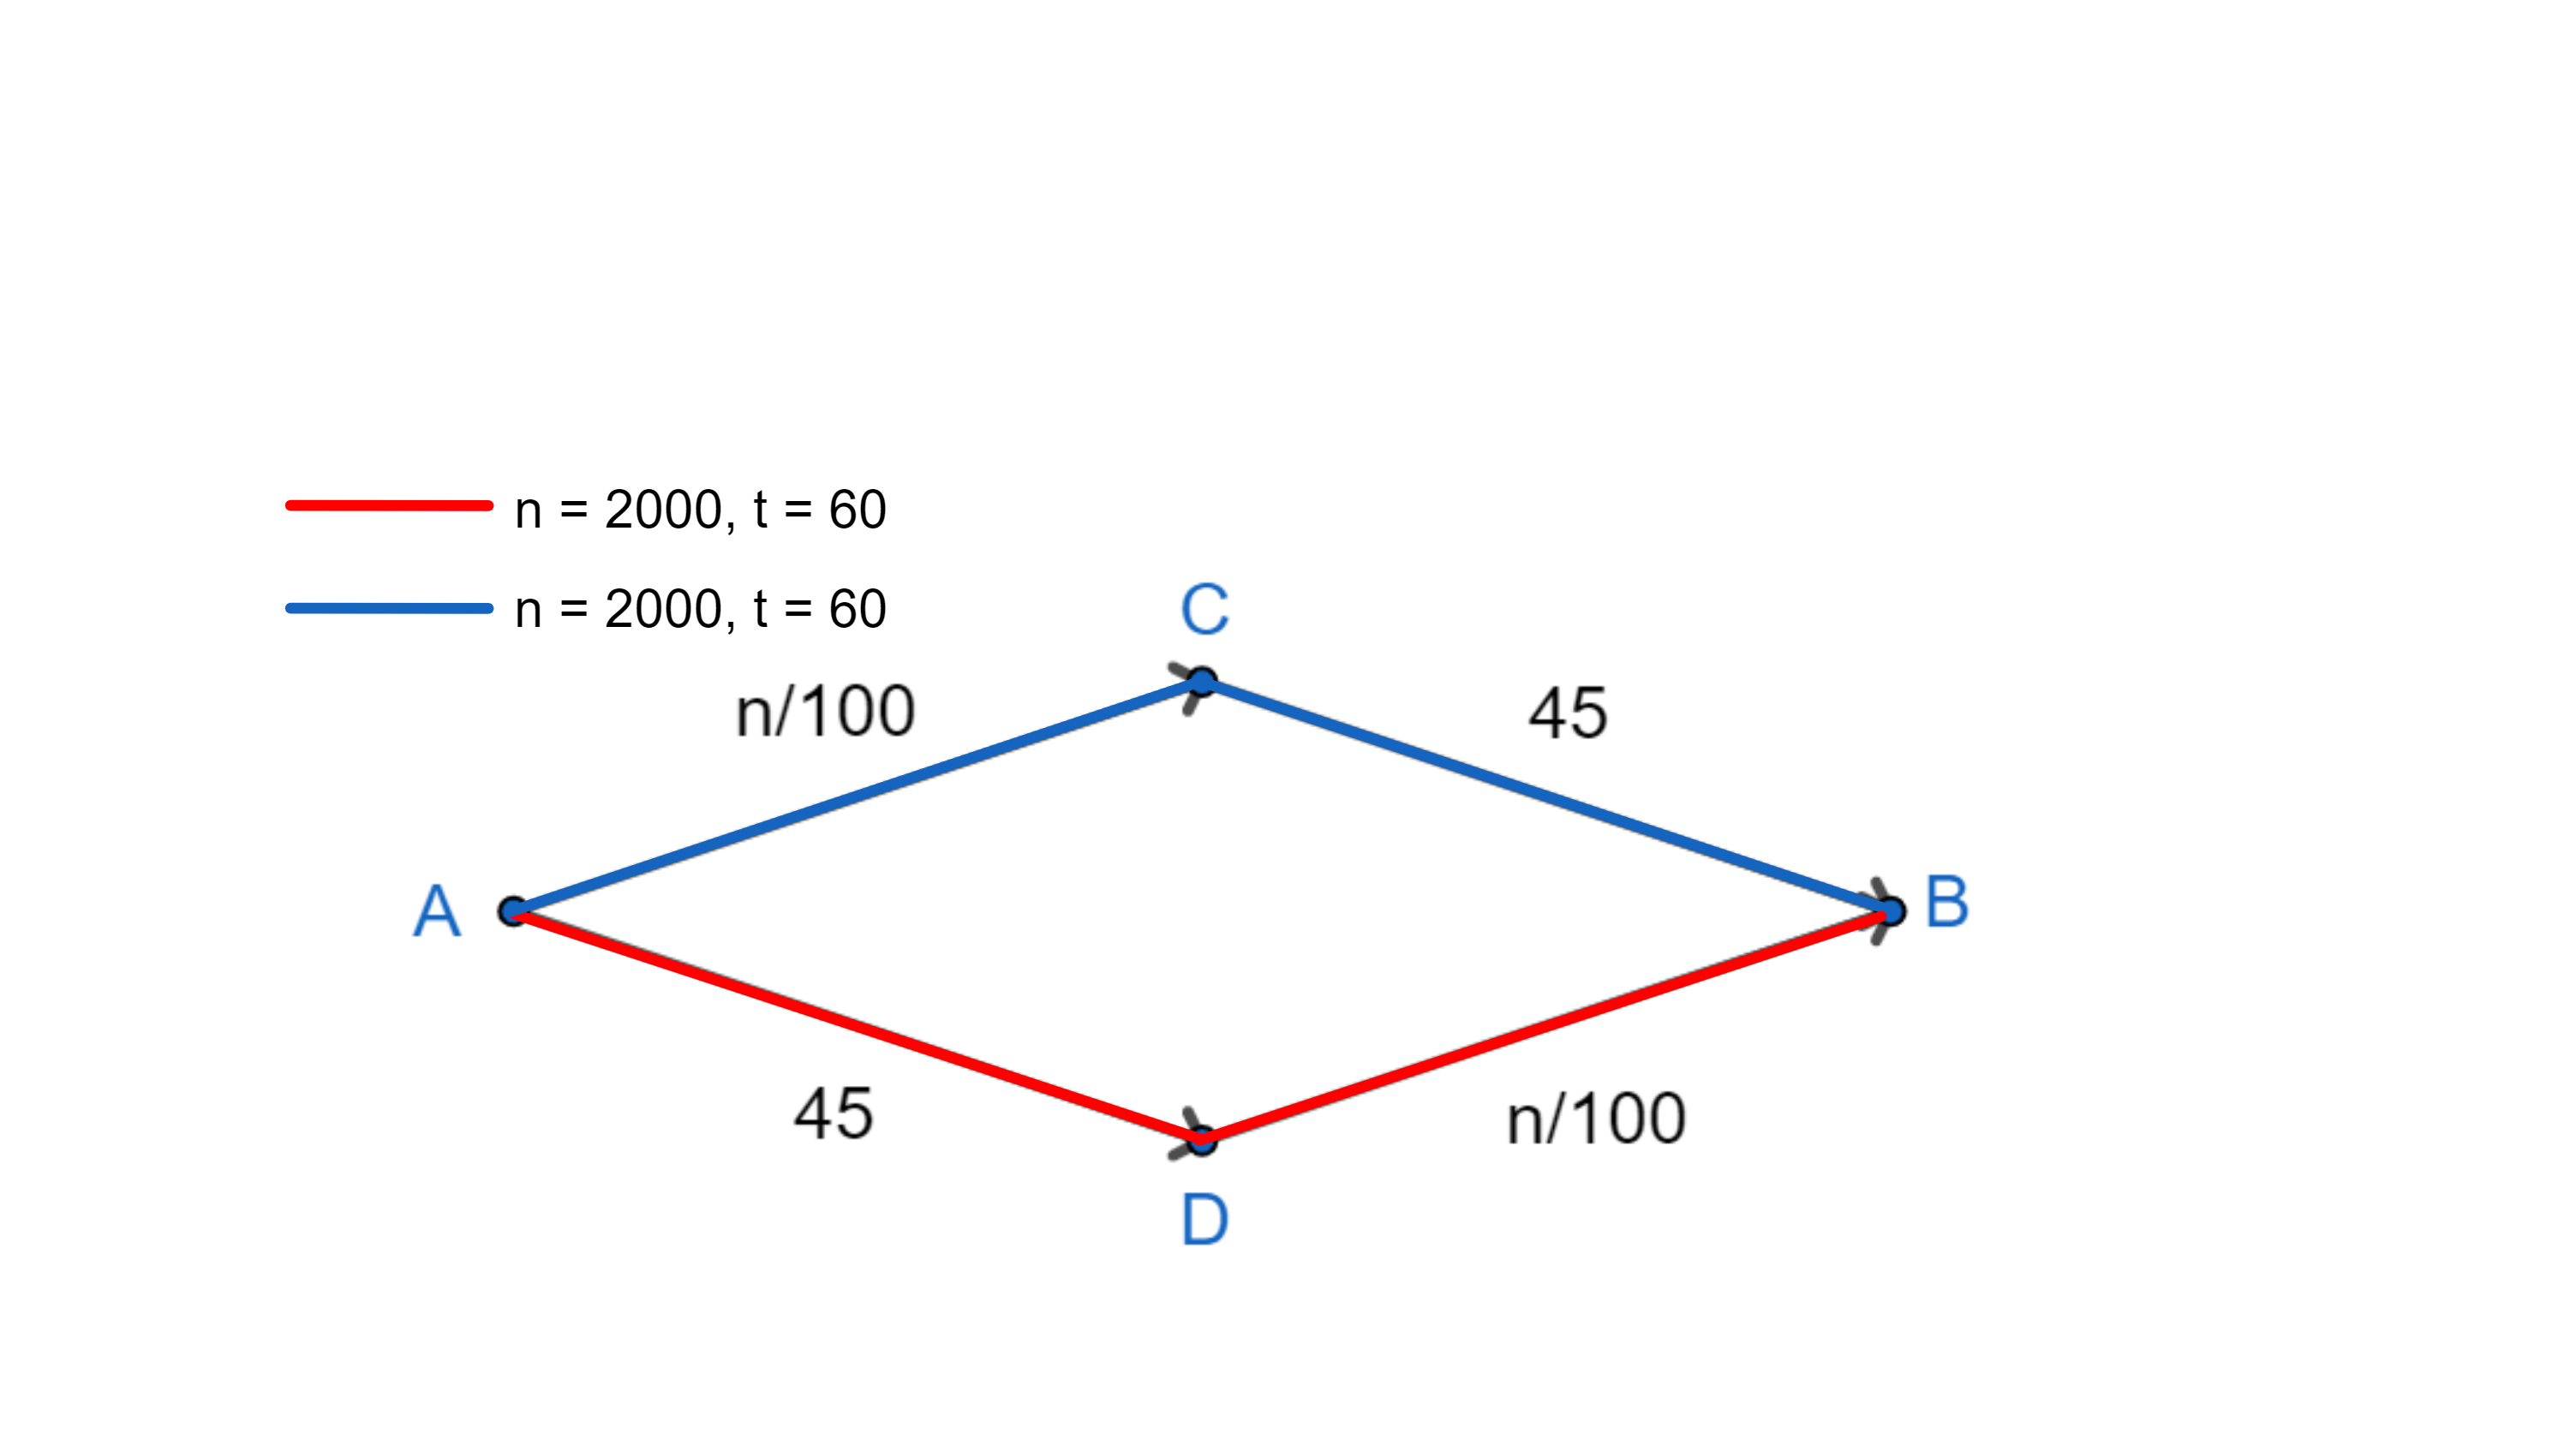
\includegraphics[width=1\linewidth]{imgs/before_braess.png}
				\caption{Оптимальное некооперативное равновесие: $2\,000$ едут по ACB, остальные по ADB. Затраты каждого $\frac{2000}{100} + 45 = 65.$}
				\label{ris:braess_1}
			\end{minipage}
			\hfill
			\begin{minipage}[h]{0.45\linewidth}
				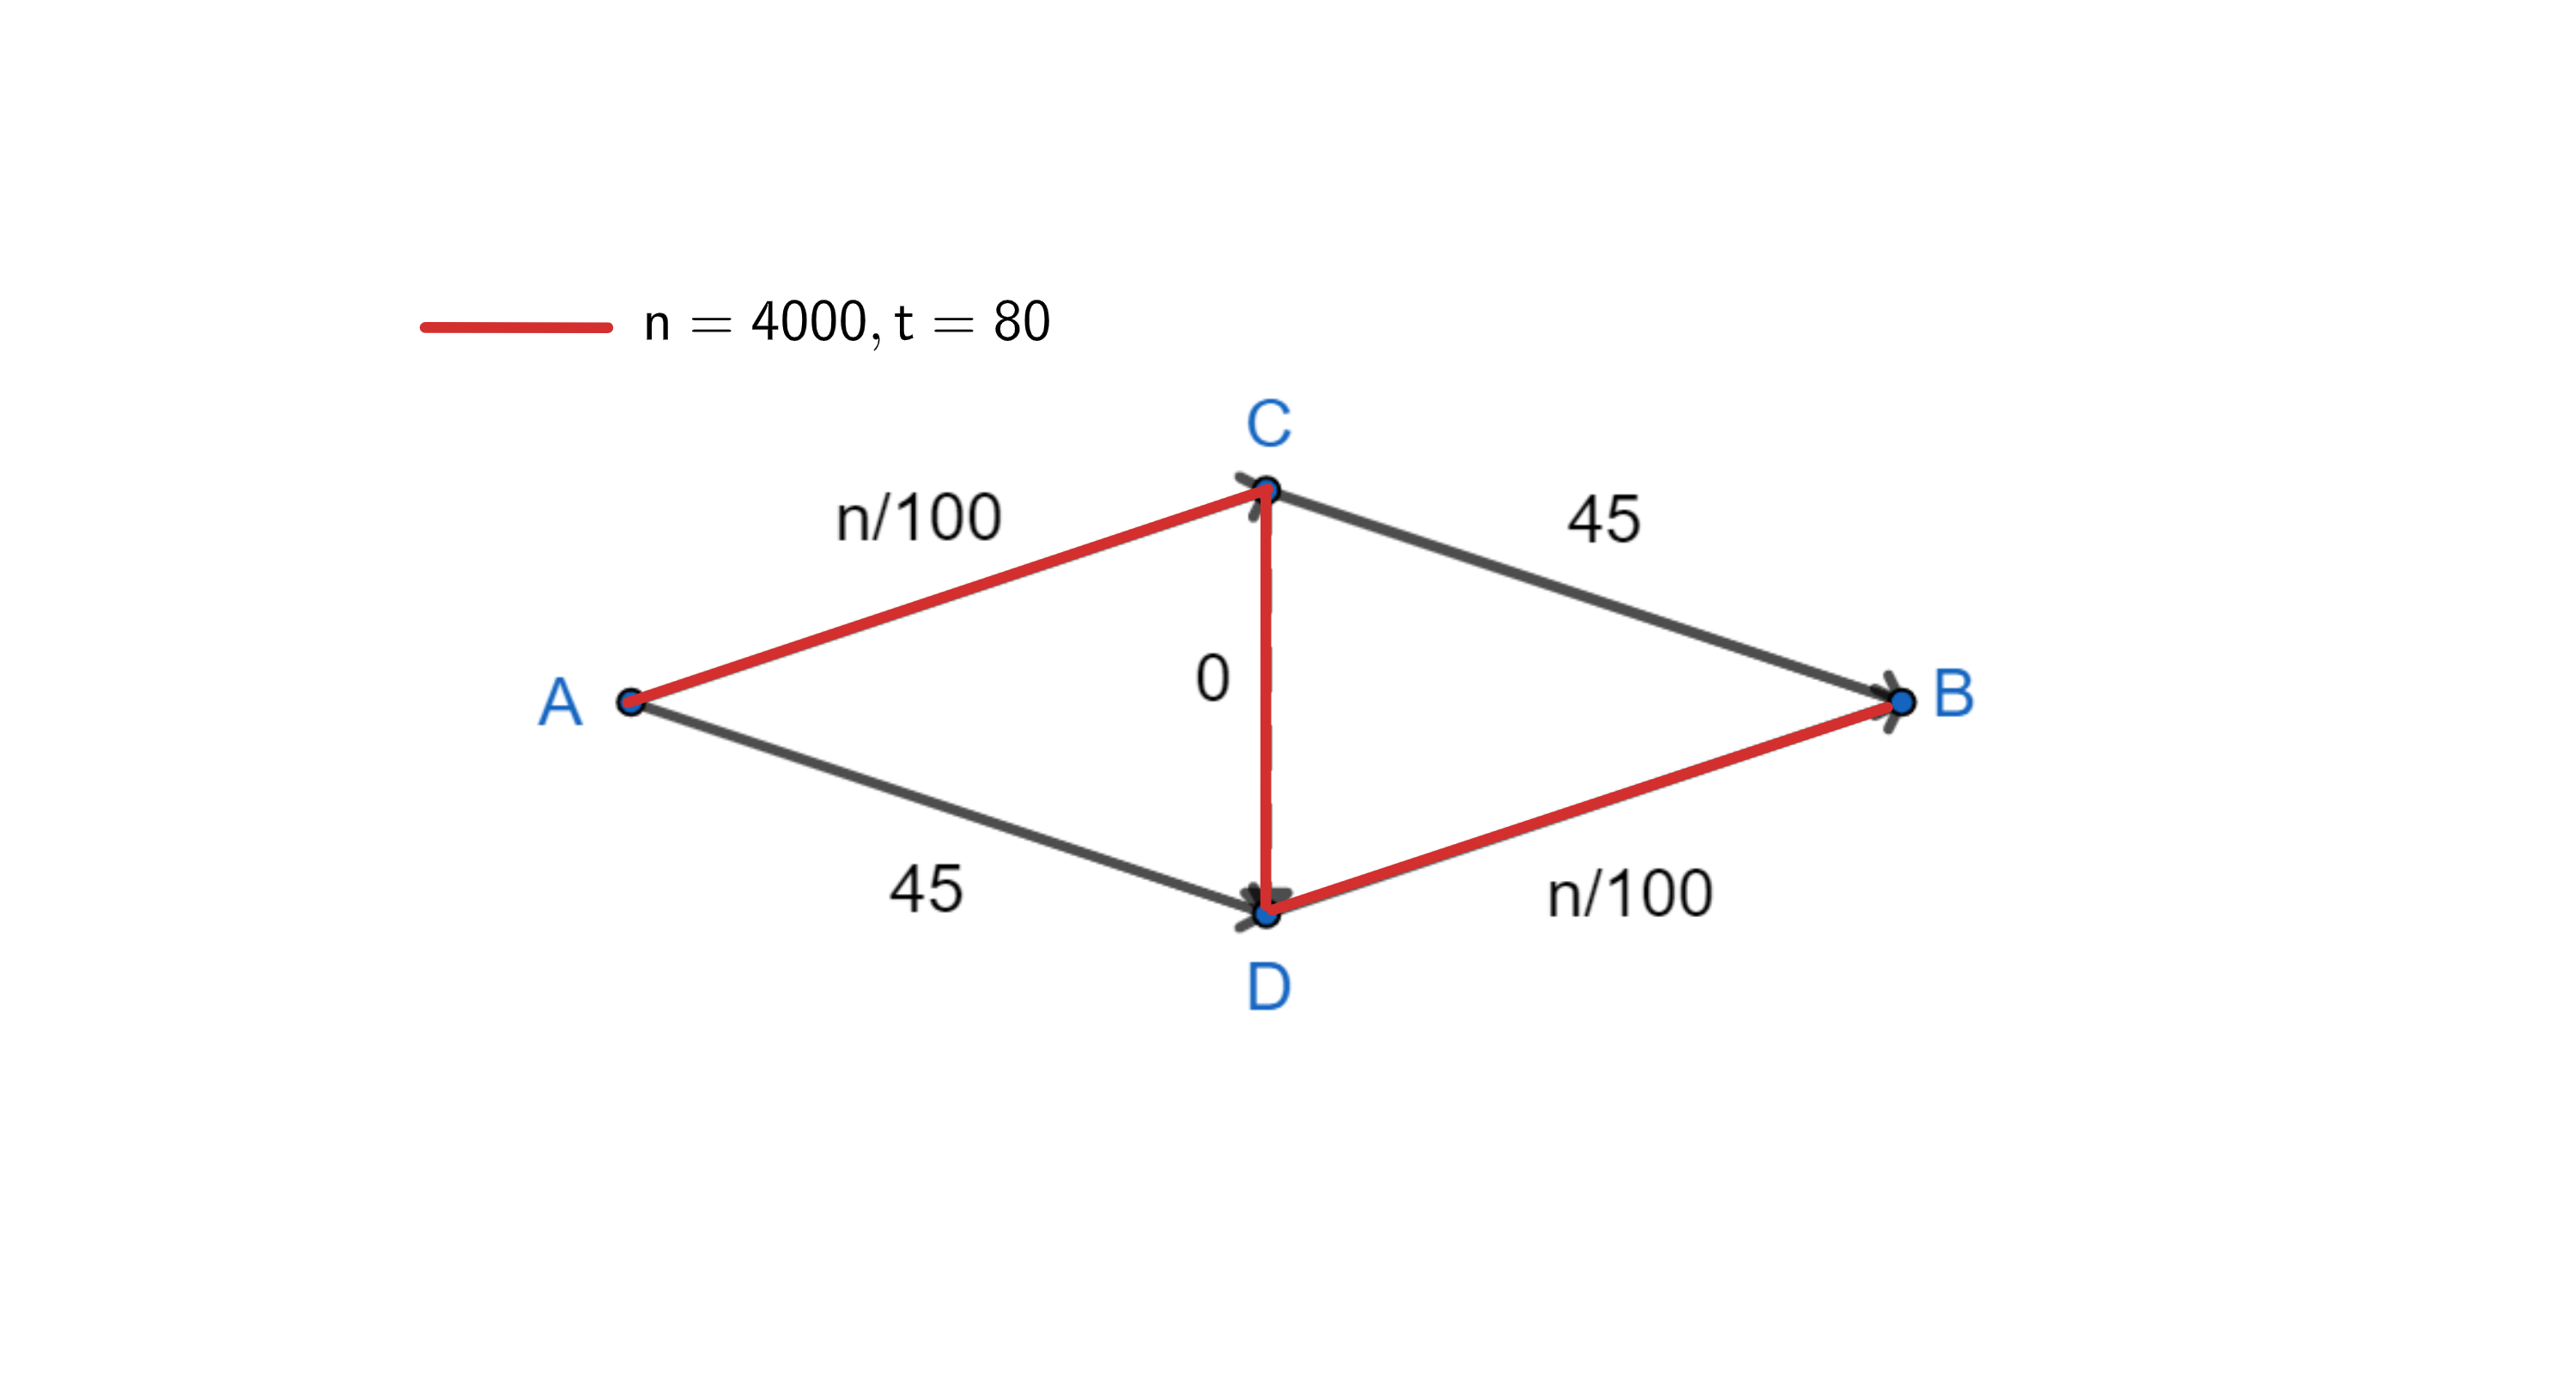
\includegraphics[width=1\linewidth]{imgs/after_braess.png}
				\caption{Добавим ребро CD. Неоптимальное некооперативное равновесие: все едут по ACDB. Затраты: 80.}
				\label{ris:braess_2}
			\end{minipage}
		\end{center}
	\end{figure}
	
\end{frame}

\begin{frame}\frametitle{Кооперативное прокладывание пути}
	Введем некоторую функцию $\Phi (\textbf{p}) = \phi (T_1 (\textbf{p}), \ldots, T_n(\textbf{p}))$, определенную на множестве всех возможных комбинаций путей $P$ и отображающую его во множество действительных чисел. С помощью нее участники могут отслеживать, как влияет изменение их пути на общую картину движения. Такую функцию назовем \textit{функцией стоимости}.
	
	\bigskip
	Для заданных некооперативного прокладывания пути $F$ и функции стоимости $\Phi$ необходимо найти комбинацию путей $\textbf{p}^*$ такую, что функция стоимости на ней минимальна, то есть
	\begin{equation}
		\Phi (\textbf{p}^*) = \minn\limits_{ \textbf{p} \in P} \Phi (\textbf{p}).
	\end{equation}
	
\end{frame}

\begin{frame}\frametitle{Примеры функции затрат}
	\begin{enumerate}
		\item  $\Phi (\textbf{p}) = \frac{1}{n}\sum\limits_{i = 1}^n T_i (\textbf{p})$ - средние временные затраты. 
		\item  $\Phi (\textbf{p}) =  T_k (\textbf{p})$ - приоритетные временные затраты.
		\item  $\Phi (\textbf{p}) = \max\limits_{i = 1, \ldots, n} T_i (\textbf{p})$ - максимальные временные затраты.
	\end{enumerate}
\end{frame}

\begin{frame}\frametitle{Проблемы практической интерпретации}
	\begin{enumerate}
		\item Как задаются функции $T_i(\textbf{p})$?
		\item Как заложено взаимодействие участников в функциях $T_i(\textbf{p})$?
	\end{enumerate}
\end{frame}


\section{Модель движения}

\begin{frame}\frametitle{Модель движения}
\textit{Модель движения} $v_i(\textbf{p}, t)$ - положительная ограниченная функция, отделенная от нуля функция, для которой верно

$$	\int\limits_{t_{e, i}^{in}(\textbf{p})}^{t_{e, i}^{out}(\textbf{p})} v_i(\textbf{p}, t) dt = l_e, e \in p_i, i = 1, \dots, n.$$

$t_{e, i}^{in}(\textbf{p}), t_{e, i}^{out}(\textbf{p})$ - неизвестные функции моментов вьезда на ребро $e$ участником $i$.
\end{frame}

\begin{frame}\frametitle{Моделирование движения}
\begin{theorem}
	Для заданной модели движения $v_i(\textbf{p}, t)$ существует единственный набор функций $t_{e, i}^{in}(\textbf{p}), t_{e, i}^{out}(\textbf{p}), T_i(\textbf{p})$ - моменты перехода между ребрами и время нахождения в пути участником $i$ соответственно, для которых верно
	
	$$T_i(\textbf{p}) = \sum \limits_{e \in p_i} t_{e, i}^{out}(\textbf{p}) - t_{e, i}^{in}(\textbf{p}).$$
\end{theorem}

Поиск таких функций называется \textit{моделированием движения}.
\end{frame}

\begin{frame}\frametitle{Проблемы практической интерпретации}
\begin{enumerate}
	\item \sout{Как задаются функции $T_i(\textbf{p})$}?
	\item \sout{Как заложено взаимодействие участников в функциях $T_i(\textbf{p})$}?
	\item Как задаются функции $v_i(\textbf{p}, t)$?
	\item Как заложено взаимодействие участников в функциях $v_i(\textbf{p}, t)$?
\end{enumerate}
\end{frame}

\begin{frame}\frametitle{Правила движения}

Имеем некоторую информацию о текущем состоянии (скорости, положения на графе, ускорения и тд.) и правилах его изменения:
\begin{enumerate}
	\item Тормозим, если впереди идущий слишком близко к нам.
	\item Ускоряемся, если впереди идущий достаточно далеко от нас.
	\item Не превышаем скорость.
	\item Тормозим перед поворотом.
\end{enumerate}
Значения функции $v_i(\textbf{p}, t)$ могут быть посчитаны применением правил движения в момент моделирования.

\end{frame}

\section{Примеры моделей движения}

\begin{frame}\frametitle{Макроскопические модели движения}
	Все определяется количеством участников на текущем ребре (плотность потока):
	$$v_i(\textbf{p}, t) = \sum \limits _{e \in E} \theta_{e, i} (\textbf{p}, t) v (n_e (\textbf{p}, t)), \; i = 1, \dots, n,$$
	где
	$$\theta_{e, i} (\textbf{p}, t) = \textbf{1}_{[t_{e, i}^{in} (\textbf{p}), t_{e, i}^{out} (\textbf{p})]} (t), \textit{ --- индикатор проезда по ребру}$$
	$$ n_{e}(\textbf{p}, t) = \sum\limits_{i = 1}^n\theta_{e, i}(\textbf{p}, t) \textit{ --- количество участников на ребре}$$
\end{frame}

\begin{frame}\frametitle{Примеры макроскопических моделей движения}
\begin{enumerate}
	\item $v (k) = \frac{v_{max}}{k}$.
	\item $v (k) = v_{max} (1 - \frac{k}{n})$.
	\item Некоторая положительная последовательность $\{v(k)\}_{k = 1}^n$.
\end{enumerate}
\vspace{10px}
	Плюс: Малая сложность моделирования.
	
	Минус: Плохо описывает реальное движение участников. 
	
\end{frame}

\begin{frame}\frametitle{Поиск оптимальной комбинации путей в макроскопических моделях движения}
	\begin{theorem}
		Пусть модель движения $ v_i(\textbf{p}, t)$ макроскопическая и функция затрат $\phi$ - линейная. Тогда задача поиска оптимальной комбинации путей есть задача смешанного целочисленного линейного программирования.
	\end{theorem}

  \bigskip
Сведение требует экспоненциального числа переменных.
\end{frame}

\begin{frame}\frametitle{Микроскопические модели движения}
\textit {Микроскопическими} называются модели движения, которые не являются макроскопическими. В таких моделях явно исследуется движение каждого автомобиля.
	
В качестве примера рассмотрим движение по бесконечному ребру. Пусть ${x_i(t) \in [0, +\infty)}$~--- координаты участника $i$. Предположим, что скорости участников ограничены некоторой общей величиной $v_{max}$. Пусть в момент времени ${t = 0}$ выполняется $x_1(0) \le x_2(0) \le \dots \le x_n(0)$.
\end{frame}

\begin{frame}\frametitle{Модель пропорциональной скорости}
Рассмотрим модель, в которой скорость участника пропорциональна расстоянию до впереди идущего участника.
Положим $d_{i} (t) = x_{i + 1} (t) - x_{i} (t), \; i = 1, \dots, n - 1$.
Без ограничения общности считаем, что $d_{i} (0) < D, \; i = 1, \dots, n - 1$, где $D$ --- расстояние, на котором происходит взаимодействие участников. Иначе рассмотрим подпоследовательности участников, для которых выполняется это условие.

Модель движения, задающуюся уравнением
\begin{equation}
	\label{eq:micro}
	v_i(t)=
	\begin{cases}
		v_{max}, & i = n,
		\\
		v_{max} \frac{d_i(t)}{D} ,& i \ne n,
	\end{cases}
\end{equation}
назовем \textit{моделью пропорциональной скорости}.
\end{frame}

\begin{frame}\frametitle{Модель пропорциональной скорости}
	
	Для поиска функций $x_i(t)$ достаточно рассмотреть систему дифференциальных уравнений
	$$ \dot{d_i} (t) = v_{i + 1} (t) - v_i (t).$$
	
	Плюс: Хорошо описывает реальное движение участников.
	Минус: Решением такой системы является
	$$d_{n - k} (\tau) = \sum \limits_{l = 0} ^ {k - 1} \left(\frac{d_{n - k + l} (0) - D}{l!} \tau^l e ^ {-\tau}\right) + D ,$$ где ${\tau = \frac{v_{max}}{D}t}$. Поэтому решение уравнения $d_{i} (t) = d_0$, необходимое в процессе моделирования может быть вычисленно только приближенно.

\end{frame}

\begin{frame}\frametitle{Модель снижения скорости}
	
Предположим, что существует некоторая величина $c_n$, которая отвечает за последовательное снижение скорости участников относительно их порядка:
$$v_{n - k} = v_{max} - c_n k, \; k = 0, \dots, n - 1.$$

\vspace{10px}
Плюс: Малая сложность моделирования.

Минус: Не использует расстояние до впереди идущей машины.
	
\end{frame}

\section{Равновесие транспортных потоков}

\begin{frame}\frametitle{Равновесие для микроскопических моделей}
	Возможность сведения микроскопических моделей к задаче MILP зависит от свойств модели. Поэтому в работе реализованы итерационные алгоритмы моделирования движения:
	\begin{itemize}    
		\item поиск неподвижной точки;
		\item алгоритм последовательного добавления участников.
	\end{itemize}
\end{frame}


\begin{frame}\frametitle{Некооперативная игра. Равновесие Нэша}
\begin{itemize}
\item \textit{Некооперативной игрой в нормальной форме} назовем тройку $\Gamma = (n, \{S_i\}_{i = 1}^n, \{H_i\}_{i = 1}^n)$, где $n \in \mathbb{N}$ --- количество участников игры, $S_i$ --- множество стратегий участника $i \in {1, \dots, n}$, $H_i$ --- функция выигрыша участника $i$, определенная на множестве ситуаций $S = \prod\limits_{i = 1}^n S_i$ и отображающая его во множество действительных чисел.
\item \textit{Равновесием Нэша} некооперативной игры в нормальной форме $\Gamma = (n, \{S_i\}_{i = 1}^n, \{H_i\}_{i = 1}^n)$ назовем стратегию $\textbf{s}^* = (s^*_1,\dots, s^*_n) \in S$ такую, что ни одному игроку $i$ невыгодно изменение своей стратегии с $s_i^*$ на любую другую $s \in S_i$:
$$H_i(\textbf{s}^*) \ge H_i(\left(s^*_1, \ldots, s^*_{i - 1}, s, s^*_{i + 1}, \ldots, s^*_{n} \right)), \; \forall s \in S_i, \; \, i = 1, \dots, n. $$ 
\end{itemize}
\end{frame}

\begin{frame}\frametitle{Кооперативное равновесие}
\begin{itemize}
\item \textit{Кооперативным равновесием} некооперативного прокладывания пути $F$ и функции стоимости $\Phi (\textbf{p})$ назовем комбинацию путей $\widetilde{\textbf{p}} \in P$, которая является равновесием Нэша некооперативной игры $\widetilde{\Gamma} = (n, \{P_i\}_{i = 1}^n, \{-\Phi\}_{i = 1}^n)$. Множество всех кооперативных равновесий обозначим $\widetilde{P}$
\end{itemize}

\begin{block}{Утверждение} 
Множество кооперативных равновесий $\widetilde{P}$ не пусто, причем
оптимальная комбинация путей является таким равновесием, то есть $\textbf{p}^* \in \widetilde{P}$.
\end{block}

\end{frame}

\begin{frame}\frametitle{Алгоритм поиска кооперативного равновесия}
	Считаем, что мы умеем решать задачу 
	$$\Phi (\textbf{p}) \rightarrow \min\limits_{p_i \in P_i}$$
	
	Алгоритмы поиска кооперативного равновесия:
	\begin{itemize}
		\item \textit{Поиск неподвижной точки}: последовательно решаем задачу оптимизации по каждому из путей, пока это возможно. 
		\item  \textit{Алгоритм последовательного добавления участников}: будем добавлять в нашу задачу по одному участнику и сводить их к неподвижной точке.
	\end{itemize}
\end{frame}

\section{Результаты. }
\begin{frame}\frametitle{Одинаковый приоритет участников}
\begin{figure}[H]
	\begin{center}
		\begin{minipage}[h]{0.45\linewidth}
			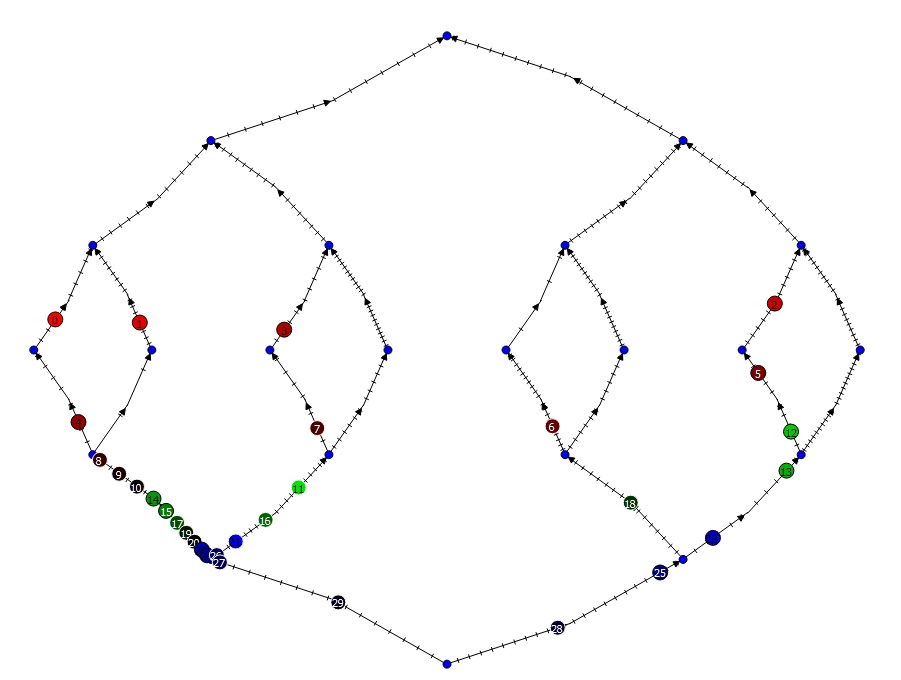
\includegraphics[width=1\linewidth]{imgs/average_good.jpg}
			\caption{Пример лучшего случая распределения путей участников в модели снижения скорости с средним временем прибытия $T = 1063$.}
		\end{minipage}
		\hfill
		\begin{minipage}[h]{0.45\linewidth}
			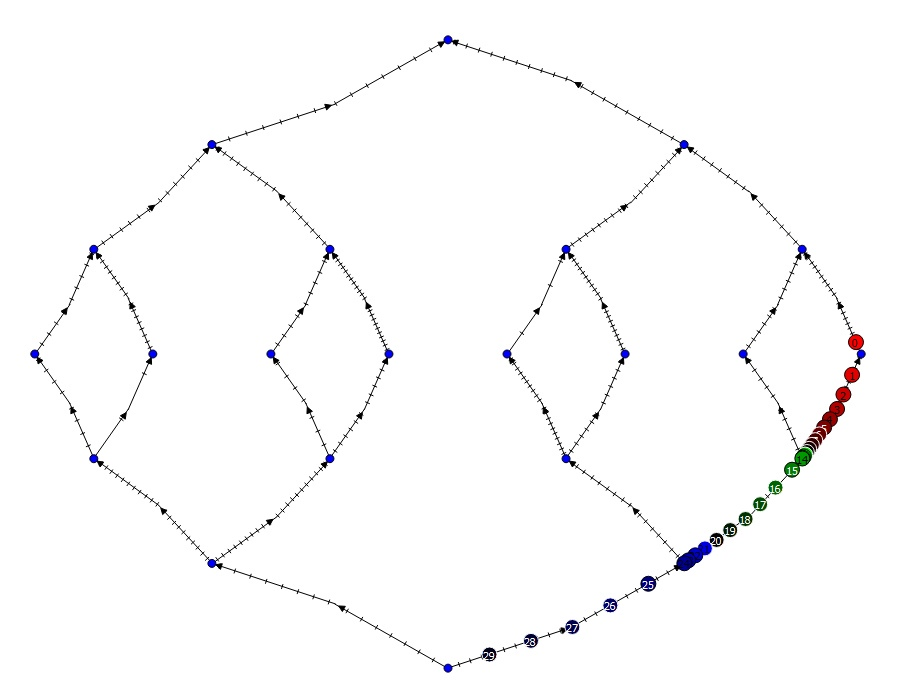
\includegraphics[width=1\linewidth]{imgs/average_bad.jpg}
			\caption{Пример худшего случая распределения путей участников в модели снижения скорости с средним временем прибытия $T = 1576$.}
		\end{minipage}
	\end{center}
\end{figure}
\end{frame}


\begin{frame}\frametitle{Поиск путей для приоритетных участников}
\begin{figure}[H]
	\begin{center}
		\begin{minipage}[h]{0.45\linewidth}
			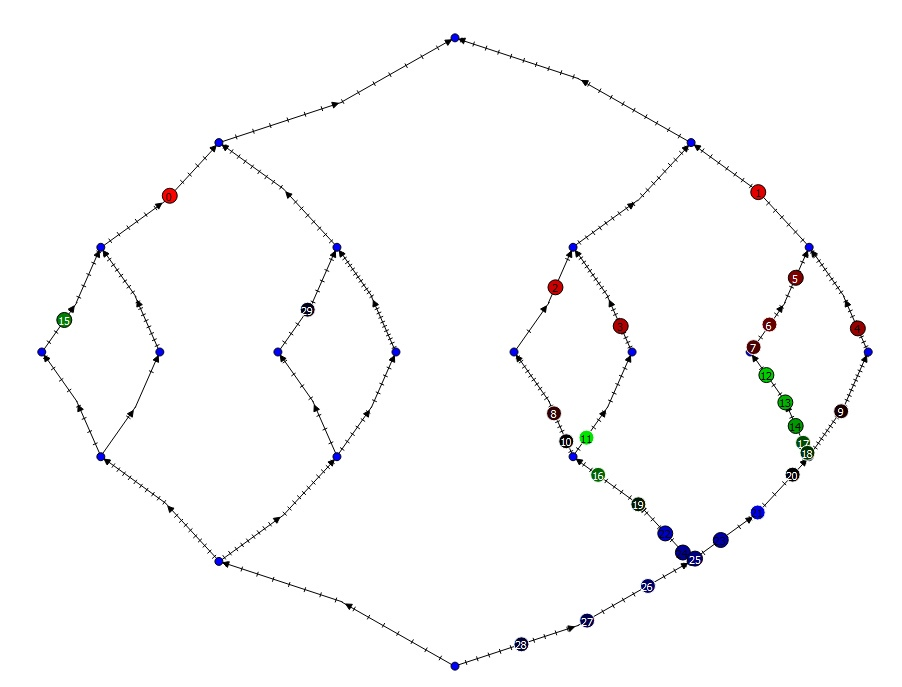
\includegraphics[width=1\linewidth]{imgs/prior_good.jpg}
			\caption{Оптимальное кооперативное равновесие в модели снижения скорости с средним временем прибытия $T = 778.34$}
		\end{minipage}
		\hfill
		\begin{minipage}[h]{0.45\linewidth}
			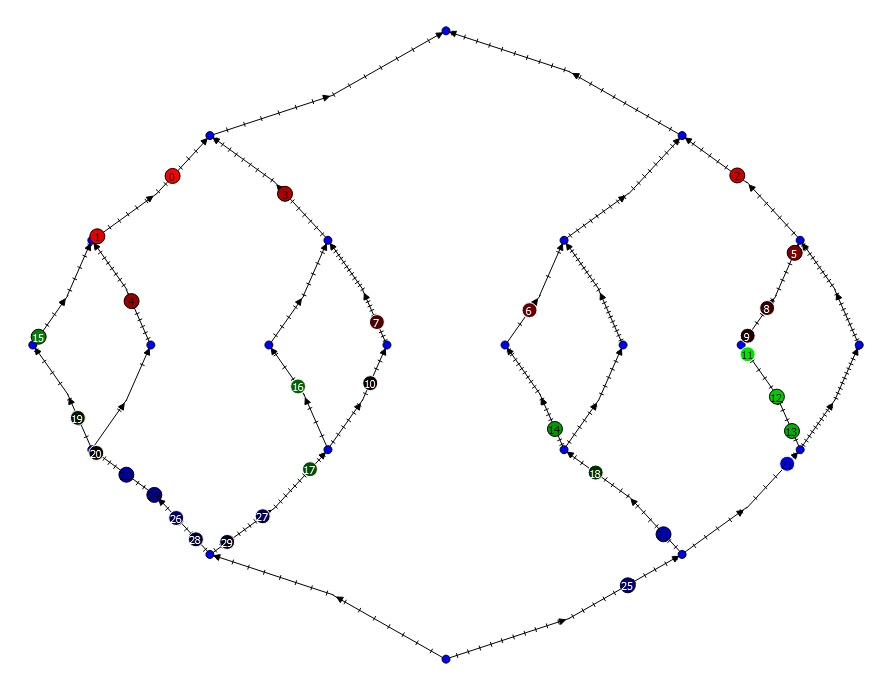
\includegraphics[width=1\linewidth]{imgs/prior_bad.jpg}
			\caption{Неоптимальное кооперативное равновесие в модели снижения скорости с средним временем прибытия $T = 950.37$ }
		\end{minipage}
	\end{center}
\end{figure}
\end{frame}

\begin{frame}\frametitle{Выводы}
	\begin{itemize}
		\item Предложено описание общего принципа взаимодействия участников, заключающегося в задании некоторой модели движения.
		\item Разработан и реализован алгоритм моделирования движения в соответствии с заданной моделью движения.
		\item Выделили класс моделей, для которого доказали возможность сведения к задаче смешанного целочисленного линейного программирования
		\item Разработаны и реализованы алгоритмы поиска корпоративного равновесия
		\item Разработоно ПО для моделирвоания, поиска оптимального пути и оптимальной комбинации путей в произвольной модели движения.
	\end{itemize}
\end{frame}

\end{document}
